%----------------------------------------------------------
\def\notedate{2022.04.25}
\def\currentauthor{Ершов В. (РК6-82Б)}
%----------------------------------------------------------
\notestatement{rndhpcedt}{Использование алгоритма DFS для решения задачи поиска циклов в ориентированном графе}

Для поиска циклов в ориентированном графе необходим алгоритм обхода графа. Обход графа - это переход от одной вершины графа к другой с целью поиска ребер или вершин, которые удовлетворяют некоторому условию.

Основными алгоритмами обхода графа являются поиск в ширину (Breadth-First Search, BFS) и поиск в глубину (Depth-First Search). Основное различие между DFS и BFS состоит в том, что DFS проходит путь от начальной вершины до конечной, а BFS двигается вперед уровень за уровнем. Из этого следует, что алгоритмы применяются для решения разных задач. BFS используется для более эффективного нахождения кратчайшего пути в графе, определения связанных компонент в графе, а также обнаружения двудольного графа. DFS применяется для проверки графа на ацикличность или для решения задачи поиска циклов в графе.

Как ранее было сказано, алгоритм DFS двигается от начальной вершины до тех пор пока не будет достигнута конечная вершина. Если был достигнут конец пути, но искомая вершина так и не была найдена, то необходимо вернуться назад (к точке разветвления) и пойти по другому маршруту. Рассмотрим работу алгоритма на примере:

\begin{figure}[H]
\center{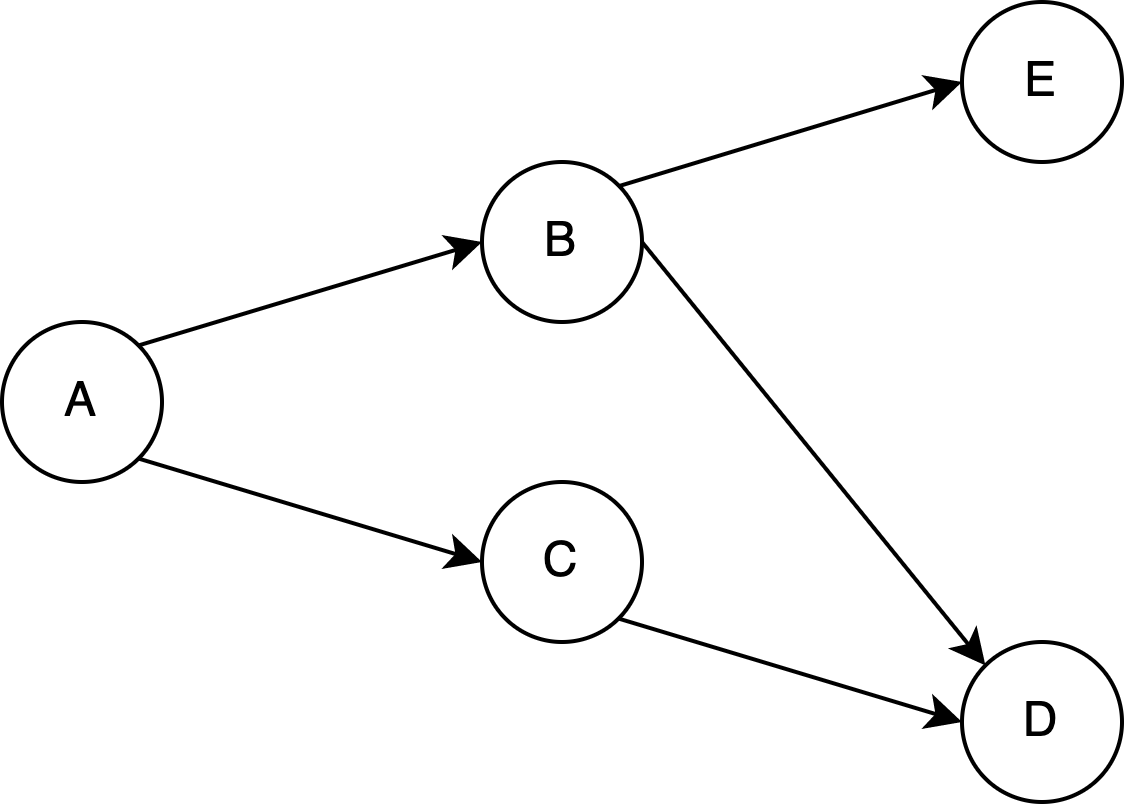
\includegraphics[width=0.7\linewidth]{ResearchNotes/rndhpc_not_edt_2022_04_25/dfs_1.png}}
\end{figure}

Мы находимся в точке ``A'' и хотим найти вершину ``E''. Согласно принципу DFS, необходимо исследовать один из возможных маршрутов до конца, если не будет обнаружена вершина ``E'', то возвращаемся и исследуем другой маршрут.

\begin{figure}[H]
\center{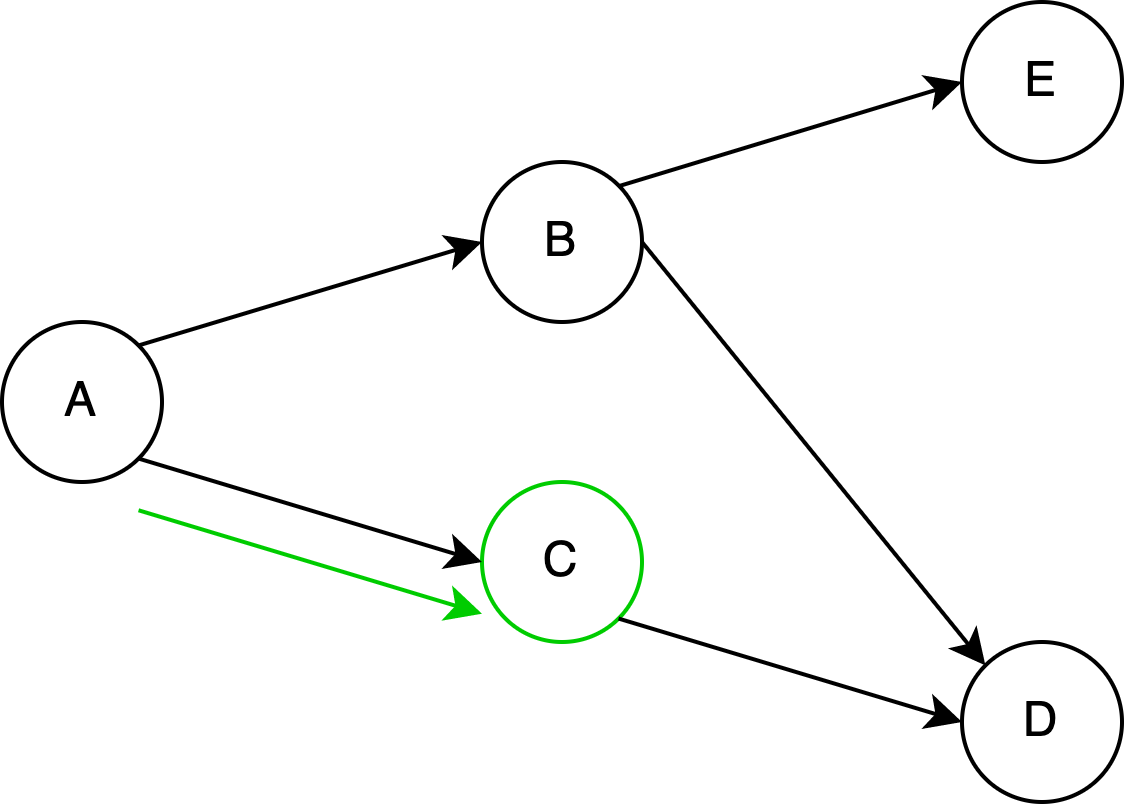
\includegraphics[width=0.7\linewidth]{ResearchNotes/rndhpc_not_edt_2022_04_25/dfs_2.png}}
\end{figure}

В данном случае мы двигаемся к ближайшей вершине ``C'', поскольку это не конец пути, то переходим к следующей вершине.

\begin{figure}[H]
\center{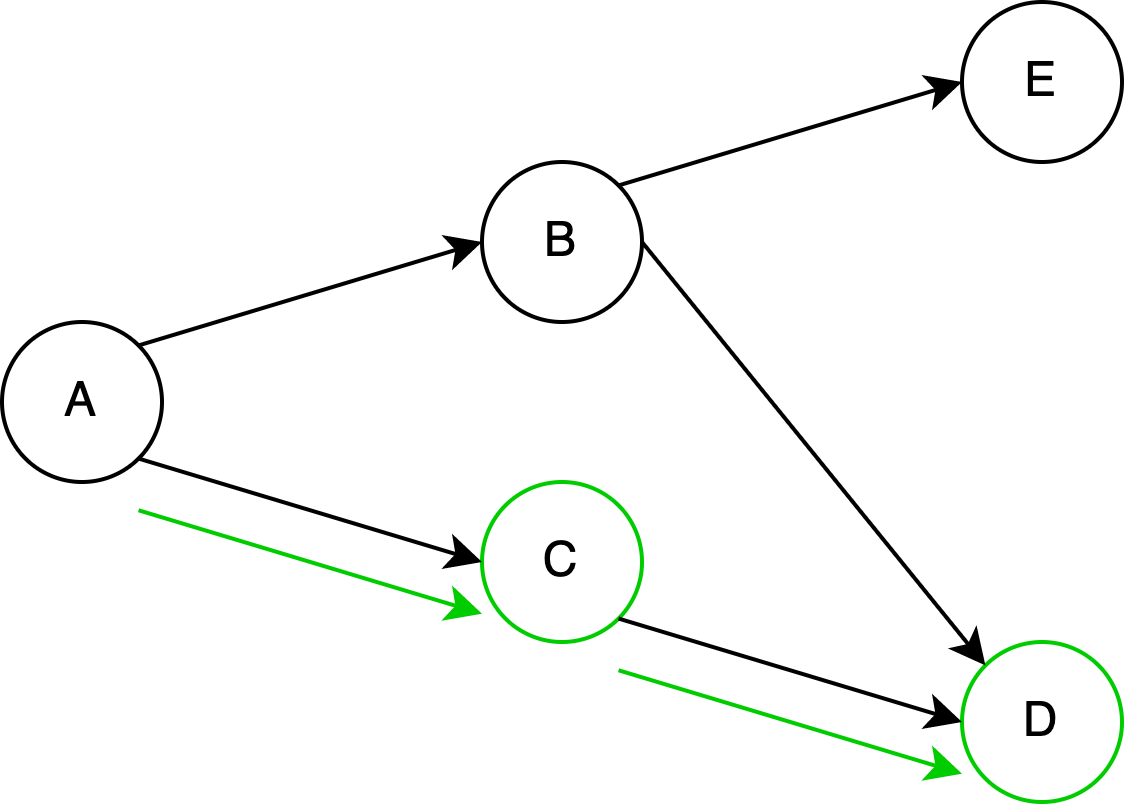
\includegraphics[width=0.7\linewidth]{ResearchNotes/rndhpc_not_edt_2022_04_25/dfs_3.png}}
\end{figure}

Мы достигли конца пути, но не нашли ``E'', поэтому возвращаемся в начальную вершину ``A'' и двигаемся по другому пути.

\begin{figure}[H]
\center{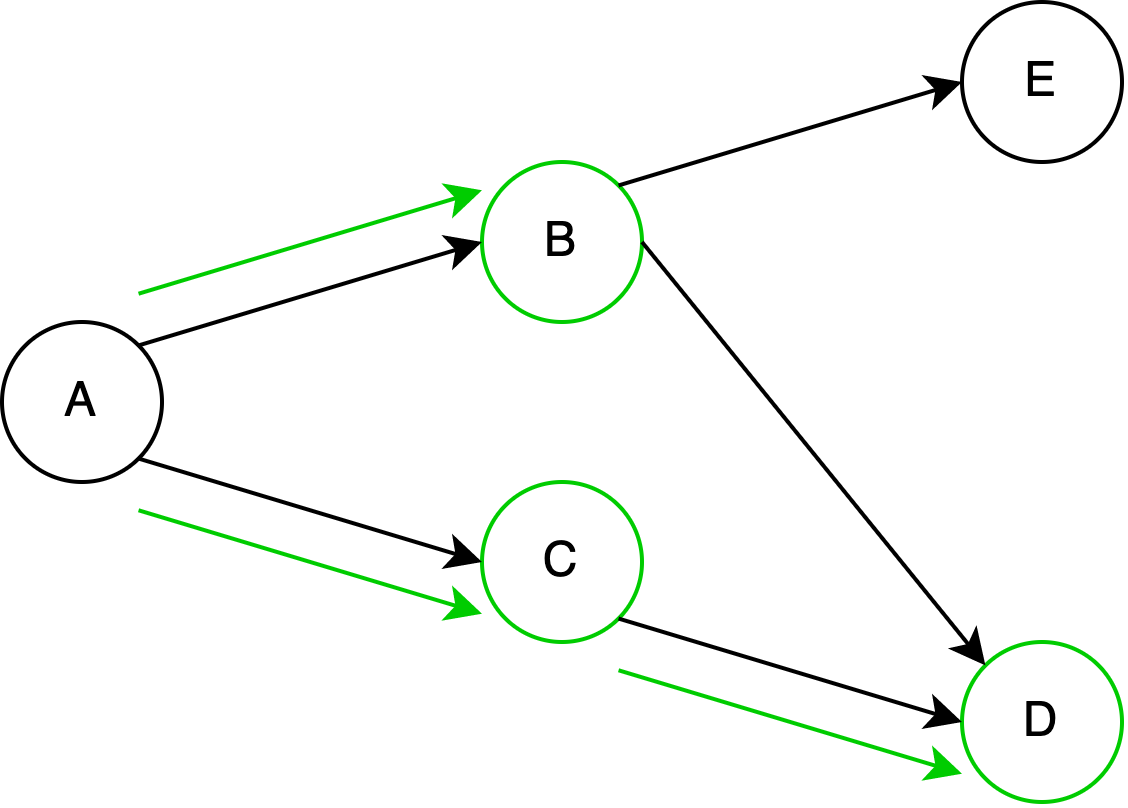
\includegraphics[width=0.7\linewidth]{ResearchNotes/rndhpc_not_edt_2022_04_25/dfs_4.png}}
\end{figure}

Из вершины ``B'' существует два возможных дальнейших пути. Поскольку вершина ``D'' была ранее расмотрена двигаемся по другому пути.

\begin{figure}[H]
\center{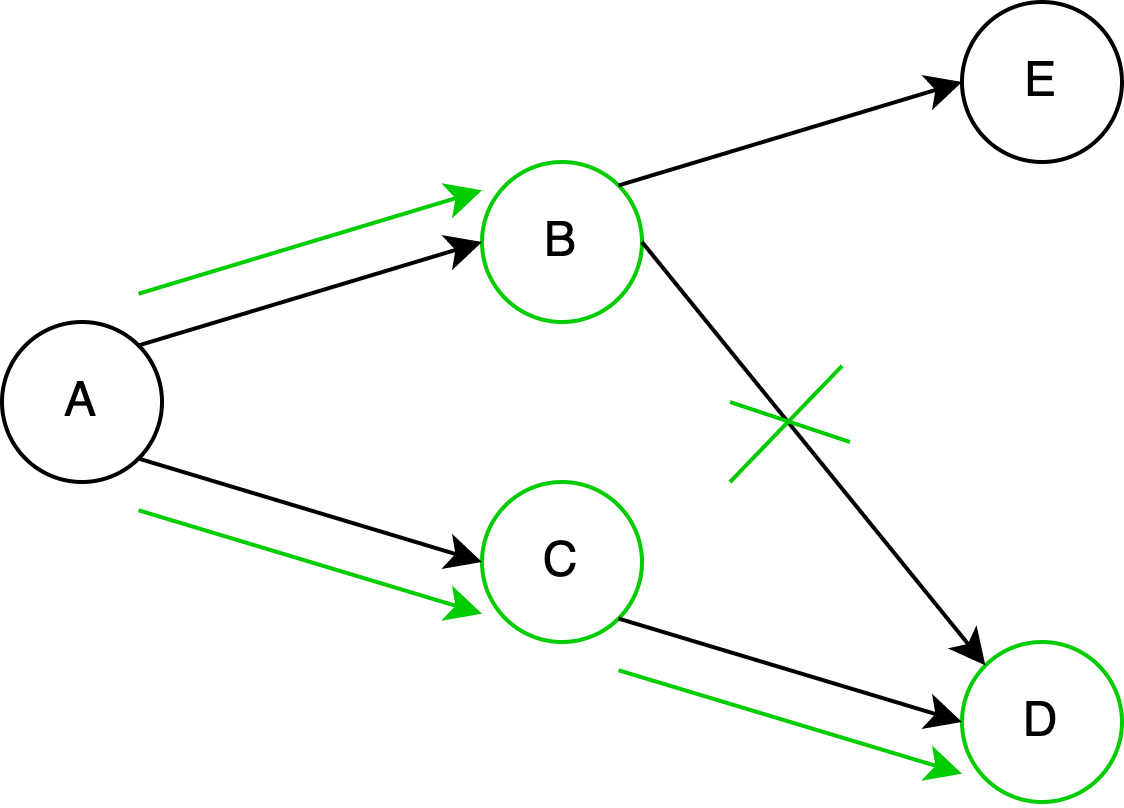
\includegraphics[width=0.7\linewidth]{ResearchNotes/rndhpc_not_edt_2022_04_25/dfs_5.png}}
\end{figure}

\begin{figure}[H]
\center{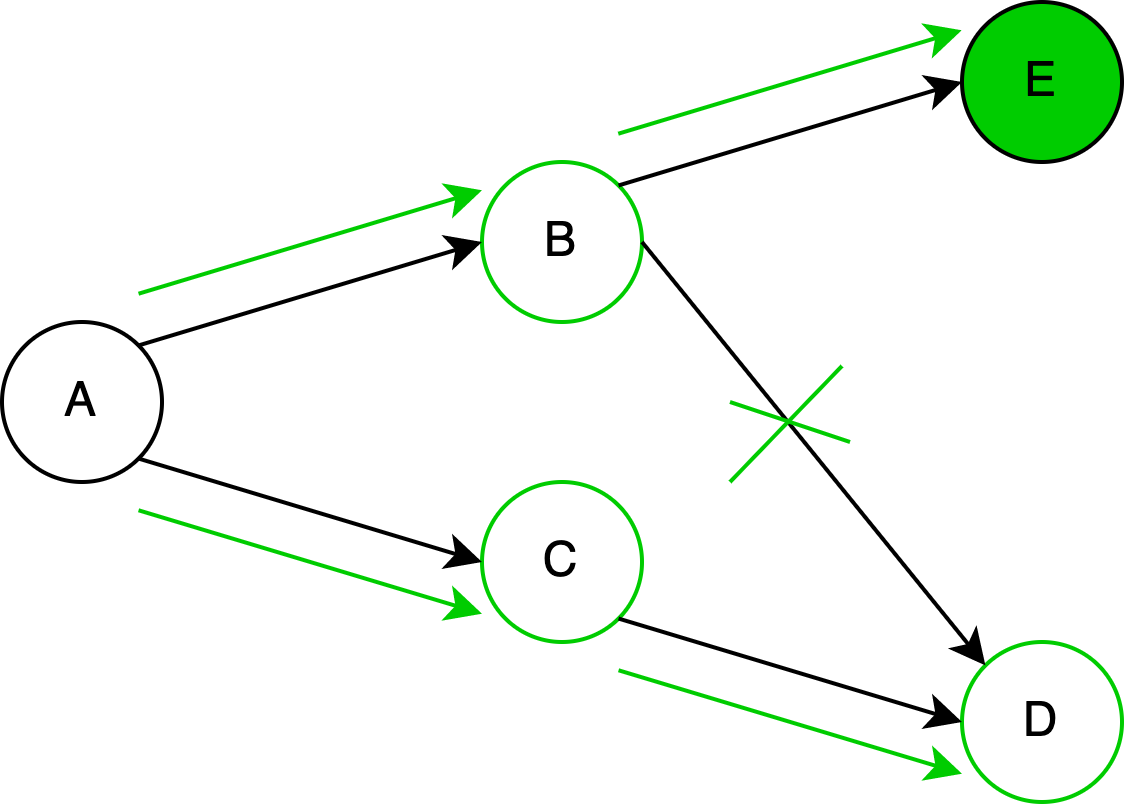
\includegraphics[width=0.7\linewidth]{ResearchNotes/rndhpc_not_edt_2022_04_25/dfs_6.png}}
\end{figure}

Мы нашли искомую вершину ``E'', следовательно можно завершать выполнение алгоритма.

В рассмотреном примере решалась достаточно тривиальная задача - поиск вершины в графе.
Более интересной является задача поиска циклов в графе. Каждая вершина графа может находиться в трех различных состояниях: вершина не посещена, вершина посещена и вершина посещена, но мы не дошли до конца пути, который включает эту вершину. Для ясности введем следующие обозначения состояний:
\begin{itemize}
	\item NOT_VISITED - вершина еще не посещена;
	\item IN_STACK - вершина посещена, но мы не дошли до конца пути;
	\item VISITED - вершина посещена.
\end{itemize}

Если в процессе обхода мы встречаем вершину, которая помечена как ``IN_STACK'', то мы нашли цикл.

В программной реализации рационально разбить задачу на три функции:
\begin{itemize}
	\item Функция, которая в цикле проходит по всем вершинам графа и если вершина не была ранее просмотрена, то запускает обход DFS из этой вершины
	\item Функция непосредственно реализующая обход DFS
	\item Функция для печати найденного цикла
\end{itemize}

Ниже приведен (листинг~\ref{lst:gm.exmpl.3}) кода данных функций на языке C++

\begin{lstlisting}[frame=single, label={lst:gm.exmpl.3}, caption={Решение задачи поиска циклов в ориентированном графе \textsf{G}}, language=C++]
void FindCycles(const std::vector<int> &adjacency_list)
{
    std::vector<std::string> visited(adjacency_list.size(), "NOT_VISITED");

    for (int vertex = 0; vertex < adjacency_list.size(); ++vertex)
    {
        if (visited[vertex] == "NOT_VISITED")
        {
            std::stack<int> stack;
            stack.push(vertex);
            visited[vertex] = "IN_STACK";
            processDFS(adjacency_list, visited, stack);
        }
    }
}

void processDFS(const std::vector<int> &adjacency_list,
                std::vector<std::string> &visited,
                std::stack<int> &stack)
{
    for (const int &vertex : adjacency_list[stack.top()])
    {
        if (visited[vertex] == "IN_STACK")
        {
            printCycle(stack, vertex);
        }
        else if (visited[vertex] == "NOT_VISITED")
        {
            stack.push(vertex);
            visited[vertex] = "IN_STACK";
            processDFS(adjacency_list, visited, stack);
        }
    }

    visited[stack.top()] = "DONE";
    stack.pop();
}

void printCycle(std::stack<int>& stack, int vertex)
{
    std::stack<int> stack_temp;
    stack_temp.push(stack.top());
    stack.pop();

    while (stack_temp.top() != vertex)
    {
        stack_temp.push(stack.top());
        stack.pop();
    }

    while (!stack_temp.empty())
    {
        std::cout << stack_temp.top() << ' ';
        stack.push(stack_temp.top());
        stack_temp.pop();
    }

    std::cout << '\n';
}
\end{lstlisting}

%-------------------------------------

%----------------------------------------------------------
% Атрибуты задачи
\noteattributes{}
%----------------------------------------------------------